\documentclass[11pt,reqno]{amsart}
%\documentclass[11pt,reqno]{article}

\usepackage{booktabs}
%\usepackage[draft]{graphics}

% -----------------------------------------------------------------------
\usepackage[english]{babel}

\usepackage[dvipsnames,svgnames]{xcolor}

\usepackage{amsmath, latexsym, amsthm, amsfonts,bm,amssymb,mathscinet} 
\usepackage{natbib}
\usepackage[text={5.8in,8.3in},centering]{geometry}
\usepackage{epsfig}
\usepackage[colorlinks,linkcolor=blue, citecolor=blue,urlcolor=blue]{hyperref}

%\usepackage[linesnumbered,ruled,vlined]{algorithm2e}

\usepackage{graphicx}
\graphicspath{{../smc/figs/}}

\usepackage{algorithm}
\usepackage{algpseudocode}


% -----------------------------------------------------------------------
\pagestyle{plain}

% -----------------------------------------------------------------------
\newcommand{\dd}{{\,\mathrm d}}
\newcommand{\ddd}{{\mathrm d}}
\newcommand{\si}{\sigma}
\renewcommand{\a}{\alpha}
\renewcommand{\b}{\beta}
\renewcommand{\th}{\theta}
\newcommand{\la}{\lambda}
\newcommand{\ga}{\gamma}
\newcommand{\ka}{\kappa}
\newcommand{\legeregel}{\par\vspace{1ex}\noindent}
\newcommand{\isd}{\stackrel{d}{=}}
\newcommand\Sgn{\mathop{\mathrm{Sgn}}\nolimits}
\newcommand{\eps}{\varepsilon}
\newcommand{\nphi}{\phi}
\renewcommand{\phi}{\varphi}
\newcommand{\asnaar}{\stackrel{\mathrm{a.s.}}{\longrightarrow}}
\newcommand{\pto}{\stackrel{\mathrm{p}}{\longrightarrow}}
\newcommand{\wto}{\rightsquigarrow}
\newcommand{\asto}{\stackrel{\mathrm{a.s.}}{\longrightarrow}}
\newcommand{\dto}{\stackrel{\mathrm{\scr{D}}}{\longrightarrow}}
\renewcommand{\scr}[1]{{\mathcal #1}}
\newcommand{\argmin}{\operatornamewithlimits{argmin}}
\newcommand{\argmax}{\operatornamewithlimits{argmax}}
\newcommand{\EE}{\mathbb{E}}
\newcommand{\FF}{\mathbb{F}}
\newcommand{\GG}{\mathbb{G}}
\newcommand{\PP}{\mathbb{P}}
\newcommand{\ind}{\mathbf{1}}
\newcommand{\RR}{\mathbb{R}}
\newcommand{\ZZ}{\mathbb{Z}}
\newcommand{\QQ}{\mathbb{Q}}
\newcommand{\CC}{\text{I\!\!\!C}}  
\newcommand{\NN}{\text{I\!N}}
\renewcommand{\vec}[1]{\underline{ #1}}
\newcommand{\ra}{\rightarrow}

\newcommand{\diag}[1]{\mathrm{diag}\left(#1\right)}

\renewcommand{\Pr}{\mathrm{Pr}}
\newcommand{\M}{\scr{M}}
\newcommand{\D}{\scr{D}}
\newcommand{\mb}[1]{\mathbf{ #1}}
\newcommand{\ft}[1]{\frametitle{#1}}
\newcommand{\Bm}{\begin{bmatrix}}
\newcommand{\Em}{\end{bmatrix}}
\newcommand{\bs}[1]{{\boldsymbol #1}}
%\newcommand{\T}{{\prime}}
\newcommand{\T}{{\top}}
\DeclareMathOperator{\tr}{tr}
% -----------------------------------------------------------------------
% My definitions for theorems etc.
\theoremstyle{definition}
\newtheorem{thm}{Theorem}
\newtheorem{prop}[thm]{Proposition}
\newtheorem{lem}[thm]{Lemma}
\newtheorem{cor}[thm]{Corollary}
\newtheorem{rem}[thm]{Remark}
\newtheorem{ex}[thm]{Example}
\newtheorem{defn}[thm]{Definition}
\newtheorem{ass}[thm]{Assumption}
\newtheorem{exer}{Exercise}
% -----------------------------------------------------------------------
\newcommand{\pr}{\ensuremath{{\rm P}}}
\newcommand{\prob}[1]{\ensuremath{{\rm P}\!\left( #1 \right)}}
\newcommand{\prc}[2]{\ensuremath{{\rm P}( #1 \, |\, #2)}}
\newcommand{\expec}[1]{\ensuremath{{\rm E}\mspace{-1mu}\left[#1\right]}}
\newcommand{\var}[1]{\ensuremath{{\rm Var}\!\left( #1 \right)}}
\newcommand{\cov}[2]{\ensuremath{{\rm Cov}\!\left( #1 , #2 \right)}}
\newcommand{\corr}[2]{\ensuremath{{\rho}\mspace{-1mu}\left( #1 , #2 \right)}}
\newcommand{\mean}[1]{\ensuremath{\bar{#1}}}

\newcommand{\simind}{\stackrel{\rm ind}{\sim}}
\newcommand{\simiid}{\stackrel{\rm iid}{\sim}}

\newcommand{\dN}[2]{\mathcal{N}\left(#1, #2\right)}

\newcommand{\hl}[1]{\textcolor{Sienna}{#1}}
\newcommand{\da}[1]{\textcolor{Navy}{#1}}
\newcommand{\fuchsia}[1]{\textcolor{Fuchsia}{#1}}
\newcommand{\red}[1]{\textcolor{red}{#1}}
%\newcommand{\note}[1]{{\color{Violet} #1}}

\newcommand{\solve}{\mathrm{solve}}

%% add notes via
\newcommand{\note}[1]{{\color{Sienna} #1}}

%---------------------------------------------------------------------------------------
\title{Safeguarding guiding}
\date{\today}
\author{Frank van der Meulen}
\address{Vrije Universiteit Amsterdam}
\email{f.h.van.der.meulen@vu.nl}

\author{Camilla Damina}
\address{Vrije Universiteit Amsterdam}
\email{c.damian@vu.nl}

\begin{document}
\maketitle


\section{Introduction}
Over the past two decades Sequential Monte Carlo (SMC) methods have gained increasing popularity. In this paper, we are specifically interested in state-space models using the {\it guided particle filter}.  Let  $\{X_t\}$ be the latent Markovian process and $\{Y_t\}$ denote  the  observation process ($t=0,1,2,\ldots$). Algorithm 10.5 in \cite{CP}  (restated here as Algorithm \ref{alg:guided_pf})  provides the steps of the guided particle  filter to approximate the filtering distribution, i.e.\ the distribution of $X_t \mid Y_0,\ldots, Y_t$.  The algorithm relies on choosing  mutation kernels $M_t$ and setting potentials $G_t$ equal to 
\[ G_t(x_{t-1},x_t) = f_t(y_t \mid x_t) \frac{P_t(x_{t-1}, \dd x_t)}{M_t(x_{t-1}, \dd x_t)}, 
\] where $f_t$ is the emission density at time $t$ (which we assume to exist) and $P_t$ is the Markov transition kernel for the latent process $\{X_t\}$. Implicitly, we assume $M_t$ to be chosen such that the Radon-Nikodym derivative in the preceding display is well defined. The output of the particle filter readily yields an unbiased estimator of the likelihood $\hat L$.



The Bootstrap filter is a special case where $M_t$ is chosen to equal $P_t$. However, choosing the kernel $M_t$ to take the future observation $y_t$ into account may lead to a more efficient algorithm,  for example quantified by an increased effective sample size (ESS). 
{\it Guiding}, also known as {\it twisting}, provides a generic framework to do so. The basic idea consists of choosing a {\it guiding function} $g_t$ and take $M_t$ equal to $P^g_t$, where
\[ P_t^{g_t}(x_{t-1}, \dd x_t) = \frac{P_t(x_{t-1}, \dd x_t) g_t(x_t)}{\int P_t(x_{t-1}, \dd x_t) g_t(x_t)} \]
assuming $g_t$ is such that  the denominator is finite. The Markovian process with these transition kernels will be referred to as the {\it guiding process} induced by $g_t$. Doob's $h$-transform consists of choosing the guiding function such that the guided process is in fact the process conditioned on the observation $y_t$; the corresponding guiding function will be denoted by $h_t$. It is well known that $h_t$ is only known in closed form in a few special cases.   In applications we therefore look for a ``good'' guiding function.  For sampling efficiency, it is advantageous to choose $g_t$ such that sampling from $P^{g_t}_t$ is feasible. It may however be the case that intuitively reasonable choices that facilitate easy sampling lead to the estimator  $\hat L$ having infinite variance, despite being unbiased. In Section 2 we give an example. 

In this paper we study safe-guarding the guided particle filter by replacing $g_t$ with $g_t + \epsilon$ for a (small) value of $\epsilon$. This idea has been briefly stated in some works on SMC (\cite{Guarniero2017}, \cite{Lindsten2018graphical}), without much detailed study. In our first part of this paper we consider discrete-time state space models and introduce an algorithm for choosing $\epsilon$ adaptively. We provide theoretical result to assess whether inclusion of a strictly positive $\epsilon$ leads to a decrease in $\chi^2$ divergence between $P^h$ and $P^{g+\epsilon}$ and therefore an increase in ESS. We illustrate this using numerical examples. 

In the second part of the paper we extend our results to the setting where the latent process is a continuous time process defined as solution to the stochastic differential equation (SDE)
\[ \dd X_t = b(t,X_t) \dd t+ q \dd W_t. \]
A guiding function induces a change of measure from the forward process, say this is denoted by $P$ to the measure $P^g$ of a process called the {\it guided} process. Following  work on exponential change of measure for continuous time stochastic processes (\cite{PalmowskiRolski2002}, \cite{BFFG}), under $P^g$ the process $X$ satisfies the SDE
 \[ \dd X_t = b(t,X_t) \dd t+ qq^\T r(t,X_t) \dd t + q \dd W^\circ_t, \]
with $r(t,x)=\nabla_x \log g(t,x)$ and $W^\circ$ a $P^g$-Wiener process. Similar to the discrete-time case we study the effect of changing $g$ to $g+\epsilon$. 



\subsection{Contributions}


\subsection{Outline}

\subsection{Frequently used notation}
 $\phi(x;\mu,\Sigma)$ denotes the  density of the $\scr{N}(\mu, \Sigma)$-distribution, evaluated at $x$.


\begin{algorithm}\label{alg:guided_pf}
\caption{Guided particle filter (GPF)}
\begin{algorithmic}[1]
\Statex Operations involving index $n$ must be performed for $n=1,\ldots,N$.
\State $X_0^n \sim \mathbb{M}_0(\mathrm{d}x_0)$
\State $w_0^n \leftarrow G_0(X_0^n)$ \Comment{where $G_0(x_0) := \dfrac{\mathbb{P}_0(\mathrm{d}x_0)\, f_0(y_0 \mid x_0)}{\mathbb{M}_0(\mathrm{d}x_0)}$}
\State $W_0^n \leftarrow w_0^n / \sum_{m=1}^N w_0^m$
\For{$t = 1$ \textbf{to} $T$}
    \If{$\mathrm{ESS}(W_{t-1}^{1:N}) < \mathrm{ESS}_{\min}$}
        \State $A_t^{1:N} \leftarrow \mathrm{resample}(W_{t-1}^{1:N})$
        \State $\widehat{w}_{t-1}^n \leftarrow 1$
    \Else
        \State $A_{t-1}^n \leftarrow n$
        \State $\widehat{w}_{t-1}^n \leftarrow w_{t-1}^n$
    \EndIf
    \State $X_t^n \sim M_t(X_{t-1}^{A_t^n}, \mathrm{d}x_t)$
    \State $w_t^n \leftarrow \widehat{w}_{t-1}^n \, G_t(X_{t-1}^{A_t^n}, X_t^n)$ \Comment{where}
    \Statex \hspace{2.5em} $G_t(x_{t-1}, x_t) := \dfrac{f_t(y_t \mid x_t)\, P_t(x_{t-1}, \mathrm{d}x_t)}{M_t(x_{t-1}, \mathrm{d}x_t)}$
    \State $W_t^n \leftarrow w_t^n / \sum_{m=1}^N w_t^m$
\EndFor
\end{algorithmic}
\end{algorithm}

%%%%%%%%%%%%%%%%%%%%%%%%%%%%%%%%%%%%%%%


\section{An example}
As first illustrative example to motivate our work, we consider the well-known stochastic volatility model. For $t=0,1,\ldots$ define 
\begin{equation}
\label{latent}
\begin{split}
	R_t &= \exp\left(\frac{X_t}{2}\right) U_t\\
	    X_t &= \omega + \psi X_{t - 1} + \eta W_t
\end{split},
\end{equation}
where $\{U_t\}$ and $\{W_t\}$ are independent sequences of independent $\scr{N}(0,1)$-distributed random variables. The process $\{X_t\}$ is latent, while $\{R_t\}$ is observed. 
We consider the following transformed version of the observation equation 
\begin{equation}\label{v_obs}
    V_i := \log\left(R_i^2\right) = X_i + U'_i, \quad 1 \leq i \leq n,
\end{equation}
where $U'_i := \log\left(U_i^2\right)$, $i = 1, \dots, n$.

For simplicity, assume $x_0$ is fixed and we wish to forward propagate a particle at $x_0$ in view of the observation $v_1$ at time $1$.  Let 
$P(x_0, \dd x_1)$ be the Markov kernel corresponding to  defined by
\[
  X_1 \mid X_0=x_0 \;\sim\; \mathcal{N}(\omega + \psi x_0,\; \eta^2).
\]
 The distribution of $X_1$, conditioned on $v_1$ and $x_0$ is given by the twisted kernel
 \[
  P^h(x_0, dx_1) = \frac{P(x_0, dx_1)\, h(x_1)}{\int P(x_0, dx_1)\, h(x_1)},\]
where 
\[
  h(x_1) = \text{density of } X_1 + \log Z^2 \text{ evaluated at } v_1,
  \quad \text{where } Z \sim \mathcal{N}(0,1).
 \]
 It is easily verified that 
% We have   \[
%  P\!\left(X_1 + \log Z^2 \le v\right)
%  = P\!\left(Z^2 \le e^{v - X_1}\right)
% \]
%so
\[
  h(x_1) = f_{\chi^2(1)}\!\left(e^{v_1-x_1}\right) e^{v_1-x_1},
\]
with $f_{\chi^2(1)}$ denoting the density of the $\chi^2(1)$-distribution. 
%For large $x_1$ it will behave like
%$\sqrt{e^{v-x_1}}$.  It should also behave this way for large $x_1$.

 As sampling from $P^h$ is non-trivial, we use a Gaussian approximation to the distribution of $\log Z^2$ to obtain the guiding function $g$ defined by 
\[
  g(x_1) = \phi(v_1;\; \mu + x_1,\; \sigma^2), \] where $\mu := \EE \log Z^2\approx -1.27$ and $\sigma^2 := \var{\log Z^2}= \pi^2/2$. \note{double check}
This induces the twisted measure
\[   P^g(x_0, \dd x_1) = \frac{P(x_0, \dd x_1)\, g(x_1)}{\int P(x_0, \dd x_1)\, g(x_1)}.
\]
Contrary to $P^h$, sampling from $P^g$ is easy. A simple calculation reveals that 
\[ P^g(x_0, \dd x_1) \sim \dN{\mu^\star}{(\sigma^\star)^2}, \]
with
\[ (\sigma^\star)^2=\frac{\eta^2\sigma^2}{\eta^2+\sigma^2} \qquad \text{and} \quad \mu^\star = \frac{\sigma^2(\omega+\psi x_0)+\eta^2(v-\mu)}{\eta^2+\sigma^2}. 
\]
\note{look up where this has been proposed in the literature and cite this}


Suppose $X_1^1,\ldots, X_1^N$ are sampled independently from $P^g(x_0, \dd x_1)$. An unbiased estimator for the likelihood is given by
\[ \hat{L} := \frac1{N}\sum_{n=1}^N G(x_0, X_1^n). \] 

\begin{prop}
	result when the second moment is finite or not
\end{prop}



Define $c_g = \int P(x_0, dx_1)\, g(x_1)$ and similarly $c_h$. As $x_0$ is fixed in this section, we omit it from our notation.  In our specific case
\[ c_g = \phi(v; \mu+\omega+\psi x_0; \sigma^2+\eta^2). \]
Moreover, 

The measure obtained from $g_\eps$ is a mixture:
\[ P^{g+\varepsilon}(x_0, d x_1) = \frac{g(x_1) + \eps}{c_g +\eps} P(x_0, dx_1) = \lambda_g(\eps) P^g(x_0, d x_1) + (1-\lambda_g(\eps)) P(x_0, d x_1), \]
with $\lambda_g(\eps)= c_g/(c_g+\eps)$. 





\section{General setup}


Consider discrete-time nonlinear Gaussian model
\[ X_{t+1} \mid X_t=x \sim \dN{b_t(x)}{Q_t(x)}. \]
Assume to observe 
\[ V_{t} \mid X_{t}=x \sim K(x,\cdot), \]

Consider the continuous-time SDE model
\[	  \dd X_t = b(t,X_t) \dd t + q \dd W_t,\qquad  X_0=x_0 .\]
Assume to observe 
\[ V_{i} \mid X_{t_i}=x \sim K(x,\cdot). \]
We  assume the Markov kernel $K$ to admit a density $k(x,\cdot)$ with respect to Lebesgue measure. 


Outline:
\begin{enumerate}
	\item focus on filtering using SMC
	\item Upon linear approximation of $b$ and $k$, we can compute guiding functions
	\item Analyse behaviour of resulting guided process, show need of safeguarding using $\eps$. 
\end{enumerate}

\section{Discrete example setup}

\section{Sequential Monte Carlo Approach}

Suppose we do sequential Monte Carlo to sample from $X_1 \mid v$ and to find
the marginal likelihood $p(v)$, which is actually $c_h$.  We use mutation kernel $M = P^{g+\eps}$.
Then it follows from the results in Chapter 5 of Chopin-Papaspiliopoulos that the 
 potential should be
\begin{align*}
G_\eps(x_1)
  & := h(x_1)\,\frac{P(x_0, dx_1)}{P^{g+\eps}(x_0, dx_1)}
  \\ & = h(x_1)\,\frac{\int P(x_0, dx_1)\, g(x_1)\, dx_1+ \eps}{g(x_1)  + \eps}
  \\ &= h(x_1)\,\frac{c_g+ \eps}{g(x_1)+ \eps} .
\end{align*}
The estimator for the marginal likelihood is
\[
 \hat{L}:= \frac{1}{N}\sum_{n=1}^{N} G_\eps\!\left(X_1^{(n)}\right),
  \qquad \bigl(X_1^{(n)}\bigr)_{n=1}^{N} \sim P^{g+\eps}(x_0, dx_1).
\]
For {\it any} $\eps>0$
\[  \EE_{P^{g+\eps}} \hat{L}=\EE_{P^{g+\eps}} G_\eps(X_1) = \int  h(x_1)\,\frac{P(x_0, dx_1)}{P^{g+\eps}(x_0, dx_1)} P^{g+\eps}(x_0, dx_1) =c_h. \]


\subsection{Analysis of variance of $\hat L$}
Define
\[
  m(\eps) = \mathbb{E}_{P^{g+\eps}}\!\left[G_\eps(x_0, X_1)\right]^2.
\]
By expanding we get
\begin{equation}\label{eq:m_eps1}
\begin{split}
  m(\eps)
  &= \int h(x_1)^2 \left(\frac{c_g+\eps}{g(x_1)+\eps}\right)^{\!2}
    \frac{P(x_0, dx_1)\,(g(x_1)+\eps)}{c_g+\eps}
  \\ &= \bigl(c_g+\eps\bigr)\int \frac{h(x_1)^2}{g(x_1)+\eps}\,P(x_0,dx_1).
	\end{split}	
\end{equation}
Define \[  I(\eps)= \int \frac{h(x_1)^2}{g(x_1)+\eps}\,P(x_0,dx_1)\] and
\[ \bar{m}(\eps) = \log m(\eps) = \log (c_g+\eps) + \log I(\eps). \]
Note that we can evaluate $c_g$ and $I(\epsilon)$ numerically using Gauss-Hermite quadrature. 



Note that we can rewrite to
\[
  I(\eps) = \int h(x_1)\,\frac{\int h(x_1)\,P(x_0,dx_1)}{g(x_1)+\eps}\;
      P^h(x_0,dx_1)
  = c_h\int \frac{h(x_1)}{g(x_1)+\eps}\,P^h(x_0,dx_1).
\]
though we won't use this expression in the numerics. 

\subsection{Infinite variance case}
Suppose $\eps=0$. 
Since $c > 0$, finiteness of $\bar{m}(0)$ is equivalent to finiteness of
\[
  I(0) = \int \frac{h(x_1)^2}{g(x_1)}\,P(x_0,dx_1).
\]



Using $f_{\chi^2(1)}(u) = (2\pi u)^{-1/2} e^{-u/2}$ we get
\[
  h(x_1) = \frac{1}{\sqrt{2\pi}}\,e^{-(v-x_1)/2}\,e^{-e^{v-x_1}/2},
\]
so
\[
  h(x_1)^2 = \frac{1}{2\pi}\,e^{-(v-x_1)}\,e^{-e^{v-x_1}}.
\]
Writing $t = x_1 - v$, the integrand of $I(0)$ equals
\[
  \frac{h(x_1)^2}{g(x_1)}\,p(x_1\mid x_0)
  \;\propto\;
  \exp\!\left(t - e^{-t} + \frac{(t+\mu)^2}{2\sigma^2}
  - \frac{(t - (\omega+\psi x_0 - v))^2}{2\eta^2}\right).
\]

We analyse the tails:
\begin{itemize}
	\item {\it Right tail $t\to+\infty$.}
The term $e^{-t}\to 0$, and expanding the quadratics the dominant behaviour is
\[
  \exp\!\left(t^2\!\left(\frac{1}{2\sigma^2} - \frac{1}{2\eta^2}\right) + O(t)\right).
\]
This is integrable if and only if the coefficient of $t^2$ is strictly negative, i.e.
\[
  \frac{1}{2\sigma^2} - \frac{1}{2\eta^2} < 0 \iff \eta^2 < \sigma^2.
\]

\item {\it Left tail $t\to-\infty$.}
The term $e^{-t}\to+\infty$ dominates inside the exponent, sending the integrand
to zero faster than any polynomial. Hence the left tail never causes divergence.
\end{itemize}

Therefore,
\begin{prop}
With the observation scheme $v = X_1 + \log Z^2$, $Z\sim\mathcal{N}(0,1)$, we have
\[
  I(0) = \int \frac{h(x_1)^2}{g(x_1)}\,P(x_0,dx_1) < \infty
  \iff \eta < \sigma.
\]
\end{prop}
It follows that for $\eta<\pi/\sqrt{2}\approx 2.221$ no regularisation is needed. For $\eta=\sigma$ the integral diverges (though like $e^t$), while for $\eta>\sigma$ divergence is much faster. 


\begin{center}
	
\includegraphics[scale=0.5]{mbar_plot_1.0.png}
\end{center}

\begin{center}
	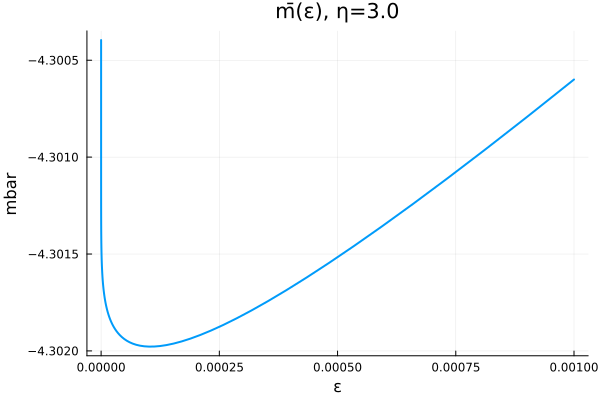
\includegraphics[scale=0.5]{mbar_plot_3.0.png}
\end{center}

\newpage


\section{Importance Sampling Quality: KL and $\chi^2$ Divergences}

\subsection{General theory}

The natural divergences for assessing IS  quality of $\hat L$ are the KL divergence and the
$\chi^2$ divergence between the target $P^h$ and the proposal $P^{g+\varepsilon}$:
\begin{align*}
  \mathrm{KL}(P^h \| P^{g+\varepsilon})
    &= \int \log\frac{dP^h}{dP^{g+\varepsilon}}\,dP^h, \\
  \chi^2(P^h \| P^{g+\varepsilon})
    &= \int \left(\frac{dP^h}{dP^{g+\varepsilon}}\right)^{\!2} dP^{g+\varepsilon} - 1.
\end{align*}
Since \[\frac{dP^h}{dP^{g+\varepsilon}}(x_1) = \frac{h(x_1)/c_h}{(g(x_1)+\eps)/(c_g+\eps)} = \frac{G_\eps(x_1)}{c_h},\] we have
\[
  \chi^2(P^h \| P^{g+\varepsilon}) =  \frac{m(\varepsilon)}{c_h^2} - 1,
\]
so finite variance of the IS estimator is \emph{exactly equivalent} to
$\chi^2(P^h \| P^{g+\varepsilon}) < \infty$. The $\chi^2$ divergence thus directly
controls the variance. Note, using $\log x \le x-1$ (and thus $2\log x \le x^2-1$)
\[  2 \mathrm{KL}(P^h \| P^{g+\varepsilon}) \le \int \left(\frac{dP^h}{dP^{g+\varepsilon}}\right)^{\!2} dP^{h} - 1  .\] \note{Original bound I wrote down was wrong.}

\subsection{KL divergence: explicit form}
We have
\begin{align*}
  \mathrm{KL}(P^h \| P^{g+\varepsilon})
  &= \log\frac{c_g+\varepsilon}{c_h}
     + \int \log h(x_1)\,P^h(x_0,dx_1)
     - \int \log(g(x_1)+\varepsilon)\,P^h(x_0,dx_1).
\end{align*}
As $\varepsilon\downarrow 0$ each term has a finite limit provided
$\int |\log g(x_1)|\,P^h(x_0,dx_1) < \infty$.
Since $\log g(x_1)$ is quadratic in $x_1$ (as $g$ is Gaussian), this requires
$P^h$ to have finite second moments. Hence
\[
  \mathrm{KL}(P^h \| P^{g+\varepsilon}) \to \mathrm{KL}(P^h \| P^g) < \infty
  \quad \text{as } \varepsilon\downarrow 0,
\]
whenever $P^h$ has finite second moments, which holds for any $\varepsilon \geq 0$
in our specific example.

\subsection{$\chi^2$ divergence and finite variance: the threshold}

For any $\varepsilon > 0$, the denominator $g(x_1)+\varepsilon \geq \varepsilon > 0$
uniformly, so
\[
  m(\varepsilon) \leq \varepsilon^{-1}\int h(x_1)^2\,P(x_0,dx_1) < \infty,
\]
provided $h\in L^2(P(x_0,\cdot))$, which holds for our specific $h$.
Hence the IS estimator has finite variance for \emph{every} $\varepsilon > 0$.

At $\varepsilon = 0$ the situation is more delicate. From the tail analysis of
Section~2, the integrand $h(x_1)^2/g(x_1)$ behaves like
\[
  \exp\!\left(t^2\!\left(\frac{1}{2\sigma^2}-\frac{1}{2\eta^2}\right) + O(t)\right)
  \quad \text{as } t = x_1 - v \to +\infty,
\]
leading to the following result.

\begin{prop}
  For the observation scheme $v = X_1 + \log Z^2$, $Z\sim\mathcal{N}(0,1)$:
  \[
    \chi^2(P^h \| P^g) < \infty \iff m(0) < \infty \iff \eta < \sigma.
  \]
\end{prop}

Now
\[ ESS \approx \frac{N}{1+\chi^2(P^h \| P^{g+\eps})}. \]
So minimising $m(\eps)$ at each SMC step is equivalent to maximising ESS. 


%



\section{Numerical Experiment: Effect of $\varepsilon$ on SMC Performance}

\subsection{Setup}

We consider the hidden Markov model
\begin{align*}
  X_t \mid X_{t-1} &\sim \mathcal{N}(\omega + \psi X_{t-1},\, \eta^2), \\
  V_t \mid X_t      &= X_t + \log Z_t^2, \quad Z_t \sim \mathcal{N}(0,1),
\end{align*}
with parameters $\omega=0$, $\psi=0.9$, $\mu=-1.27$, $\sigma^2=\pi^2/2$.
We compare two regimes:
\begin{itemize}
  \item \textbf{Regime A} ($\eta=1.0 < \sigma\approx 2.22$): finite-variance
    regime, where $m(0)<\infty$.
  \item \textbf{Regime B} ($\eta=3.0 > \sigma$): infinite-variance regime,
    where $m(0)=\infty$.
\end{itemize}
In both regimes we run SMC with the twisted proposal $P^{g+\varepsilon}$ for
several values of \[ \varepsilon \in \{0, 0.001, 0.01, 0.05, 0.1\}.\]

\subsection{SMC Algorithm}

At each time step $t$, the twisted proposal is the mixture
\[
  P^{g+\varepsilon}(x, \cdot) =
    \frac{c(x)}{c(x)+\varepsilon}\,P^g(x,\cdot)
    + \frac{\varepsilon}{c(x)+\varepsilon}\,P(x,\cdot),
\]
where both $c(x)$ and the parameters of $P^g$ are available in closed form
(see Section~2). The IS weight for a particle $x_t$ proposed from
$P^{g+\varepsilon}(x_{t-1},\cdot)$ is
\[
  G_\varepsilon(x_{t-1}, x_t) = \frac{h_t(x_t)}{g_t(x_t)+\varepsilon}\,(c(x_{t-1})+\varepsilon).
\]

\begin{algorithm}
\caption{Guided particle filter (GPF) with twisted proposal $P^{g+\varepsilon}$,
  following \citet[Algorithm~10.5]{chopin2020introduction}}
\label{alg:gpf}
\begin{algorithmic}[1]
\Require observations $v_{1:T}$, particle count $N$, perturbation $\varepsilon\geq 0$,
  ESS threshold $\mathrm{ESS}_{\min}$
\State For $n=1,\ldots,N$: draw
  $X_0^n \sim P(x_0)$,
  set $w_0^n \leftarrow G_0(X_0^n)$,
  $W_0^n \leftarrow w_0^n / \sum_{m=1}^N w_0^m$
  \newline where $G_0(x_0) := P_0(dx_0)\,h_0(x_0)/M_0(x_0)$
\For{$t = 1, \ldots, T$}
  \If{$\mathrm{ESS}(W_{t-1}^{1:N}) < \mathrm{ESS}_{\min}$}
    \State $A_{t-1}^{1:N} \leftarrow \mathrm{resample}(W_{t-1}^{1:N})$
    \State $\hat{w}_{t-1} \leftarrow 1$
  \Else
    \State $A_{t-1}^n \leftarrow n$
    \State $\hat{w}_{t-1} \leftarrow w_{t-1}^n$
  \EndIf
  \State For $n=1,\ldots,N$: draw
    $X_t^n \sim M_t(X_{t-1}^{A_{t-1}^n},\,dx_t) = P^{g_t+\varepsilon}(X_{t-1}^{A_{t-1}^n},\,dx_t)$
    \newline by sampling from
    $P^{g_t}(X_{t-1}^{A_{t-1}^n},\cdot) = \mathcal{N}(\mu^*,\sigma^{*2})$
    with probability $\alpha^n = c(X_{t-1}^{A_{t-1}^n})/(c(X_{t-1}^{A_{t-1}^n})+\varepsilon)$,
    and from $P(X_{t-1}^{A_{t-1}^n},\cdot)$ otherwise
  \State $w_t^n \leftarrow \hat{w}_{t-1}^n \cdot G_t(X_{t-1}^{A_{t-1}^n},\, X_t^n)$
    \newline where
    \[
      G_t(x_{t-1}, x_t) :=
        \frac{h_t(x_t)}{g_t(x_t)+\varepsilon}
        \cdot\bigl(c(x_{t-1})+\varepsilon\bigr)
    \]
  \State $W_t^n \leftarrow w_t^n \,/\, \sum_{m=1}^N w_t^m$
\EndFor
\State \Return
  $\sum_{t=1}^T \log \ell_t^N$,\quad
  $\{\mathrm{ESS}(W_t^{1:N})\}_{t=1}^T$
  \newline where, following equation~(10.3) of \citet{chopin2020introduction},
  \[
    \ell_t^N :=
    \begin{cases}
      \dfrac{1}{N}\displaystyle\sum_{n=1}^N w_t^n
        & \text{if resampling occurred at time } t, \\[8pt]
      \left(\sum_{n=1}^N w_t^n\right)/\left(\sum_{n=1}^N w_{t-1}^n\right)
        & \text{otherwise.}
    \end{cases}
  \]
\end{algorithmic}
\end{algorithm}

\noindent
To assess performance, we run Algorithm~\ref{alg:gpf} independently $R=500$
times on the same simulated dataset ($T=50$, $N=2000$) and record both the minimum
ESS over time and the maximum normalised weight over time for each run. Define
\begin{align*}
  \mathrm{ESS}_{\min} &= \min_{t=1,\ldots,T} \mathrm{ESS}_t,	\\
  Q_{\max} &= \max_{t=1,\ldots,T} \max_n W^n_t.
\end{align*}
 A low $\mathrm{ESS}_{\min}$ indicates that at some point the
particle cloud collapsed to a near-degenerate distribution, with a single
particle carrying almost all the weight. similarly a large $Q_{\max}$ value indicates this. 

\subsection{Results}

Figure~\ref{fig:miness_cdf} shows the empirical CDF of $\mathrm{ESS}_{\min}$
across $R=500$ runs for each value of $\varepsilon$, separately for the two
regimes. We took $N=500$ particles for a dataset with $T=50$. 
\begin{itemize}
	\item {\it Regime A ($\eta < \sigma$).}
One can see an improvement upon taking $\epsilon>0$, though $\epsilon=0.01$ is clearly too large. One can see that the minimal ESS is about $60$ for $\epsilon=0$.   This confirms the
theoretical prediction: when $m(0)<\infty$, the IS weights have finite
variance.  While finiteness is guaranteed, it is typically beneficial to take nonzero $\eps$. The value $m(0)$ can still be large, while finite. 

\item {\it Regime B ($\eta > \sigma$).}
The picture changes dramatically. At $\varepsilon=0$ the CDF has substantial
mass near zero, meaning that in a significant fraction of runs the particle
cloud collapses to near-degeneracy at some time step. Taking 
$\varepsilon=0.01$ shifts the CDF markedly rightward, essentially eliminating
the collapses. This is the direct numerical manifestation of $m(0)=\infty$:
the IS weights have infinite variance, leading to occasional but catastrophic
weight concentration on a single particle.
\end{itemize}



\subsection{On the difficulty of choosing $\varepsilon$ in Regime B}

The results highlight that the choice of $\varepsilon$ in Regime B is
delicate. The optimal $\varepsilon^*$ exists and can in principle be found by
minimising $m(\varepsilon)$ numerically, as described in Section~3. However,
$m(\varepsilon)$ depends on $x_0$ and varies across time steps as the particle
cloud evolves, so a single fixed $\varepsilon$ cannot be globally optimal.
Furthermore, the performance is sensitive to this choice: the 5th percentile
of $\mathrm{ESS}_{\min}$ drops sharply on both sides of $\varepsilon^*$,
leaving a narrow window of well-performing values.

This suggests that a fixed $\varepsilon$ is fundamentally limited in Regime B,
and that an \emph{adaptive} scheme --- choosing $\varepsilon_t$ at each step
based on the current particle cloud by minimising an empirical estimate of
$m(\varepsilon)$ --- would be more robust. In Regime A, by contrast, $\varepsilon=0$
is already satisfactory.



\begin{figure}
	\begin{center}
		
\includegraphics[scale=0.6]{adaptive_miness_cdf_good.png}\\[.5in]
				
\includegraphics[scale=0.6]{adaptive_miness_cdf_bad.png}\\[.5in]
			\caption{minESS comparison. \label{fig:miness_cdf}}
	\end{center}
\end{figure}


\subsection{Work by Chatterjee \& Diaconis}
Suggest to look at $Q_{\max}$-statistic. See Figure \ref{fig:maxqn_cdf}. 
 is maximum of the normalised weights. Note that $Q_{\max}\in [0,1]$ and we want it to be small.  

\begin{figure}
	\begin{center}
		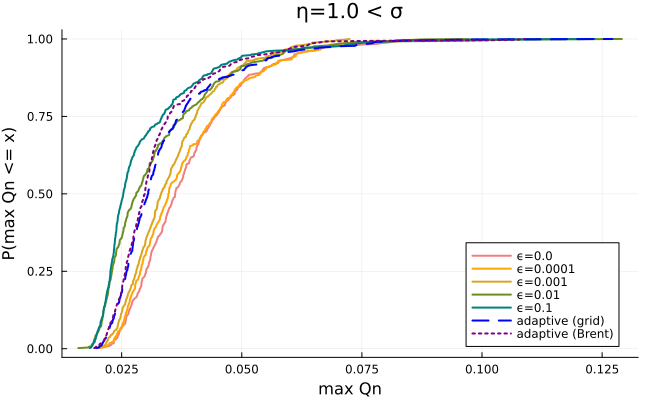
\includegraphics[scale=0.6]{adaptive_maxqn_cdf_good.png}\\[.5in]
				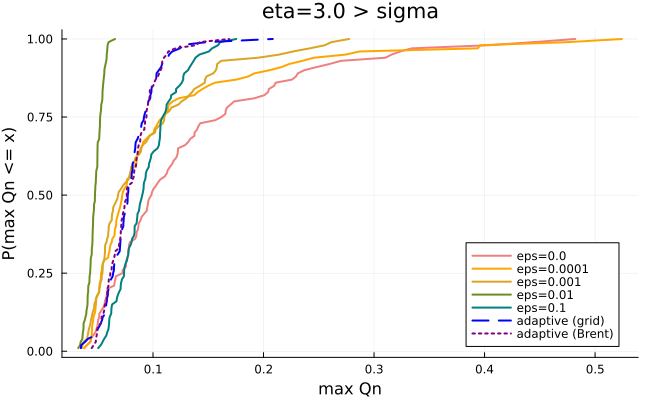
\includegraphics[scale=0.6]{adaptive_maxqn_cdf_bad.png}\\[.5in]
			\caption{Max $Q_n$ comparison.\label{fig:maxqn_cdf}}
	\end{center}
\end{figure}



%%%%%%%%%%%%%%%%%%%%%%%%%%%%%%%%%%%%%%%%%%%%%%%
\section{Adaptive Choice of $\varepsilon_t^*$}

The following result motivates the adaptive estimator. For a fixed particle
$x_{t-1}$ and observation $v_t$, under $X_t \sim P^{g_t+\varepsilon}(x_{t-1},\cdot)$, the second moment of the IS weight
equals
\[
  m(\varepsilon, x_{t-1}) =
    \bigl(c(x_{t-1})+\varepsilon\bigr)
    \int \frac{h_t(x_1)^2}{g_t(x_1)+\varepsilon}\,P(x_{t-1},dx_1).
\]
Given the particle cloud $\{X_{t-1}^n\}$ with normalised weights
$\{W_{t-1}^n\}$, the population-level second moment is the weighted average
\[
  \tilde m(\varepsilon) = \sum_{n=1}^N W_{t-1}^n \cdot m(\varepsilon, X_{t-1}^n)
  = \sum_{n=1}^N W_{t-1}^n\,\bigl(c(X_{t-1}^n)+\varepsilon\bigr)
    \int \frac{h_t(x_1)^2}{g_t(x_1)+\varepsilon}\,P(X_{t-1}^n,dx_1).
\] So we evaluate $m(\varepsilon)$  by taking the expectation of $x_{t-1}$ over the current particle approximation. 
The idea is to choose 
\[ \varepsilon_t^* = \argmin_{\varepsilon \geq 0}\, \tilde m(\varepsilon).\]
The integral appearing in $\tilde m(\eps)$ can be approximately using numerical quadrature, but in our implementation we approximate it by  drawing 
$\tilde{X}_t^n \sim P(X_{t-1}^n,\cdot)$ once and computing
\[
  \hat{m}(\varepsilon) =
    \sum_{n=1}^N W_{t-1}^n\,
    \frac{h_t(\tilde{X}_t^n)^2}{g_t(\tilde{X}_t^n)+\varepsilon}
    \cdot\bigl(c(X_{t-1}^n)+\varepsilon\bigr).
\] Thus, this is a  Monte-Carlo estimator for $\tilde m(\varepsilon)$ based on $N$ samples. 
The analytical derivative with respect to $\eps$ is
\[
  \frac{d\hat{m}}{d\varepsilon} =
    \sum_{n=1}^N W_{t-1}^n\,
    h_t(\tilde{X}_t^n)^2\,
    \frac{g_t(\tilde{X}_t^n) - c(X_{t-1}^n)}
         {(g_t(\tilde{X}_t^n)+\varepsilon)^2},
\]
which enables gradient-based optimisation. An alternative consists of minimising
$\hat{m}(\varepsilon)$ over a log-spaced grid $\mathcal{E} =
\{\varepsilon_1 < \cdots < \varepsilon_K\}$.

\begin{algorithm}
\caption{Adaptive GPF with $\varepsilon_t^*$ chosen by weighted grid search}
\label{alg:gpf_adaptive}
\begin{algorithmic}[1]
\Require observations $v_{1:T}$, particle count $N$,
  ESS threshold $\mathrm{ESS}_{\min}$,
  grid $\mathcal{E} = \{\varepsilon_1 < \cdots < \varepsilon_K\}$
\State For $n=1,\ldots,N$: draw
  $X_0^n \sim \mathcal{N}(0,\,\eta^2/(1-\psi^2))$,
  set $W_0^n \leftarrow 1/N$, $w_0^n \leftarrow 1$
\For{$t = 1, \ldots, T$}
  \State \textbf{Find $\varepsilon_t^*$:} draw auxiliary proposals
    $\tilde{X}_t^n \sim P(X_{t-1}^n,\,\cdot\,)$ for $n=1,\ldots,N$, and set
    \[
      \varepsilon_t^* = \argmin_{\varepsilon \in \mathcal{E}}\;
        \hat{m}(\varepsilon), \qquad
      \hat{m}(\varepsilon) =
        \sum_{n=1}^N W_{t-1}^n\,
        \frac{h_t(\tilde{X}_t^n)^2}{g_t(\tilde{X}_t^n)+\varepsilon}
        \cdot\bigl(c(X_{t-1}^n)+\varepsilon\bigr)
    \]
    Discard $\{\tilde{X}_t^n\}$ after this step.
  \If{$\mathrm{ESS}(W_{t-1}^{1:N}) < \mathrm{ESS}_{\min}$}
    \State $A_{t-1}^{1:N} \leftarrow \mathrm{resample}(W_{t-1}^{1:N})$,\quad
      $\hat{w}_{t-1}^n \leftarrow 1$
  \Else
    \State $A_{t-1}^n \leftarrow n$,\quad
      $\hat{w}_{t-1}^n \leftarrow w_{t-1}^n$
  \EndIf
  \State \textbf{Propose:} for $n=1,\ldots,N$ draw
    $X_t^n \sim P^{g_t+\varepsilon_t^*}\!\left(X_{t-1}^{A_{t-1}^n},\,\cdot\,\right)$
    by sampling from
    $P^{g_t}(X_{t-1}^{A_{t-1}^n},\cdot) = \mathcal{N}(\mu^*,\sigma^{*2})$
    with probability
    $\alpha^n = c(X_{t-1}^{A_{t-1}^n})/
      (c(X_{t-1}^{A_{t-1}^n})+\varepsilon_t^*)$,
    and from $P(X_{t-1}^{A_{t-1}^n},\cdot)$ otherwise
  \State \textbf{Update weights:}
    \[
      w_t^n = \hat{w}_{t-1}^n \cdot G_t\!\left(X_{t-1}^{A_{t-1}^n},\,X_t^n\right),
      \qquad
      G_t(x_{t-1},x_t) :=
        \frac{h_t(x_t)}{g_t(x_t)+\varepsilon_t^*}
        \cdot\bigl(c(x_{t-1})+\varepsilon_t^*\bigr)
    \]
  \State \textbf{Likelihood increment} (eq.~10.3 of
    \citet{chopin2020introduction}):
    \[
      \ell_t^N :=
      \begin{cases}
        \dfrac{1}{N}\displaystyle\sum_{n=1}^N w_t^n
          & \text{if resampling occurred at time }t,\\[8pt]
           \left(\sum_{n=1}^N w_t^n\right)/\left(\sum_{n=1}^N w_{t-1}^n\right)
          & \text{otherwise}
      \end{cases}
    \]
  \State \textbf{Normalise:}\quad
    $W_t^n \leftarrow w_t^n \,/\, \sum_{m=1}^N w_t^m$
  \State \textbf{ESS:}\quad
    $\mathrm{ESS}_t \leftarrow \bigl(\sum_n (W_t^n)^2\bigr)^{-1}$
\EndFor
\State \Return
  $\sum_{t=1}^T \log \ell_t^N$,\quad
  $\{\mathrm{ESS}_t\}_{t=1}^T$,\quad
  $\{\varepsilon_t^*\}_{t=1}^T$
\end{algorithmic}
\end{algorithm}

\paragraph{Remarks.}
\begin{itemize}
  \item The auxiliary proposals $\{\tilde{X}_t^n\}$ are drawn from the
    untwisted kernel $P$ and discarded after the grid search. Since they do
    not enter the weight update, the likelihood estimator
    $\sum_t \log\ell_t^N$ remains unbiased for $\log p(v_{1:T})$ for any
    data-dependent choice of $\varepsilon_t^*$.

  \item Using the carry-over weights $W_{t-1}^n$ in $\hat{m}(\varepsilon)$
    is essential when resampling has not occurred recently. After resampling
    all weights equal $1/N$ and the weighted and unweighted averages
    coincide; in steps without resampling the weight distribution can be
    skewed and the unweighted average gives a poorly-targeted
    $\varepsilon_t^*$. Numerical experiments confirm that the weighted
    version gives a substantial improvement in both min-ESS and
    $Q_{\max}$ diagnostics.

  \item The grid $\mathcal{E}$ is log-spaced over $[10^{-6}, 1]$ with $K=50$
    points. All $K$ evaluations of $\hat{m}(\varepsilon)$ reuse the same
    proposals $\{\tilde{X}_t^n\}$, so the cost is $O(KN)$ per step.
    Reducing to $K=20$ or $K=30$ would roughly halve the cost with
    negligible impact on $\varepsilon_t^*$.


\end{itemize}


%%%%%%%%%%%%%%%%%%%%%%%%%%%%%%%%%%%%%%%%%%%%%%%%%%%%%%%%%%%%%%%%%%%%%%%%%%%%%%%%
\section{Adaptive Choice of $\varepsilon$ via ESS Targeting}
\note{This does not work; I guess the desired ESS simply cannot be attained.}
\subsection{Motivation}

The numerical experiments of Section~4 show that the optimal perturbation
$\varepsilon^*$ varies across time steps and depends on the current particle
cloud. A fixed $\varepsilon$ cannot be globally optimal. We propose an
adaptive scheme inspired by tempering methods in SMC
\cite{neal2001annealed,del2006sequential}, where a tempering parameter is
chosen at each step so that the ESS after reweighting equals a target
fraction $\rho N$. The same principle applies here: we choose $\varepsilon_t^*$
such that the ESS of the IS weights equals $\rho N$.

\subsection{ESS as a Function of $\varepsilon$}

Given proposals $\{x_t^{(i)}\}_{i=1}^N$ drawn from $P(x_{t-1}^{(i)},\cdot)$,
the ESS of the weights $w^{(i)}(\varepsilon) = h_t(x_t^{(i)})/(g_t(x_t^{(i)})+\varepsilon)$
is
\[
  \mathrm{ESS}(\varepsilon) =
    \frac{\bigl(\sum_i w^{(i)}(\varepsilon)\bigr)^2}
         {\sum_i w^{(i)}(\varepsilon)^2}.
\]
Two key properties make this suitable for bisection:
\begin{enumerate}
  \item $\mathrm{ESS}(\varepsilon)$ is \emph{increasing} in $\varepsilon$:
    as $\varepsilon\to\infty$, all weights converge to $h_t(x_t^{(i)})/\varepsilon$
    and become equal, so $\mathrm{ESS}\to N$.
  \item $\mathrm{ESS}(0)$ may be small or even zero if some $g_t(x_t^{(i)})=0$,
    reflecting the weight degeneracy in the infinite-variance regime.
\end{enumerate}
The target $\varepsilon_t^*$ is therefore the unique solution of
\[
  \mathrm{ESS}(\varepsilon_t^*) = \rho N,
\]
found by bisection on $\varepsilon \in [0, \varepsilon_{\max}]$. If
$\mathrm{ESS}(0) \geq \rho N$ already, we set $\varepsilon_t^* = 0$; if even
$\varepsilon_{\max}$ is insufficient, we set $\varepsilon_t^* = \varepsilon_{\max}$.

\subsection{Connection to $m(\varepsilon)$}

The ESS targeting criterion is closely related to minimising $m(\varepsilon)$.
Note that
\[
  \frac{\mathrm{ESS}(\varepsilon)}{N}
  \approx \frac{1}{1 + \chi^2(P^h \| P^{g+\varepsilon})}
  = \frac{c_h(x_0)^2}{m(\varepsilon)},
\]
so targeting $\mathrm{ESS}(\varepsilon) = \rho N$ is equivalent to targeting
$\chi^2(P^h\|P^{g+\varepsilon}) = (1-\rho)/\rho$, i.e.\ a fixed level of the
$\chi^2$ divergence. Rather than minimising $m(\varepsilon)$ (which requires
a grid search and gives a different target at each step), ESS targeting gives
a directly interpretable, step-by-step criterion for particle diversity, and
bisection finds the solution efficiently without a grid.



\section{Conclusion}

Figure~\ref{fig:smc_single_run} shows the results of a single SMC run for
both regimes and both fixed ($\varepsilon=0$) and adaptive $\varepsilon^*$.
Even for $\eta=3$ the results with $\varepsilon=0$ can be just fine: a single
run looks almost indistinguishable from the adaptive run in terms of ESS,
cumulative log-likelihood, and incremental log-likelihood. However, if one
were to repeat the analysis many times, occasionally this would result in a
catastrophic drop in ESS. This is precisely the implication of $m(0)=\infty$:
it does not mean every run fails, but that the variance of the IS weights
across runs is infinite, so disasters occur with positive probability and
cannot be ruled out from a single run alone. This is confirmed by the CDF
plots of Figure~\ref{fig:miness_cdf}, which required $R=200$ independent
runs to reveal the heavy left tail of the min-ESS distribution at
$\varepsilon=0$.

Two further observations support this interpretation. First, the incremental
log-likelihood panel shows a pronounced dip around $t=30$ in both the fixed
and adaptive runs for $\eta=3$. This dip is driven by a particular difficult
observation and occurs regardless of $\varepsilon$, suggesting it reflects a
genuinely hard step in the data rather than an algorithmic failure. In a
catastrophic run, this dip would be far deeper and the ESS would collapse to
near 1 at that point. Second, the adaptive $\varepsilon^*$ panel for $\eta=3$
shows $\varepsilon^*$ spiking upward precisely around $t=30$, at the same
difficult observation. This confirms that the adaptive scheme is responding
correctly: it detects the hard step through the empirical minimiser of
$\hat{m}(\varepsilon)$ and automatically increases $\varepsilon$ to protect
against weight collapse, without any explicit knowledge of which observations
are difficult.

\begin{figure}
	\begin{center}
		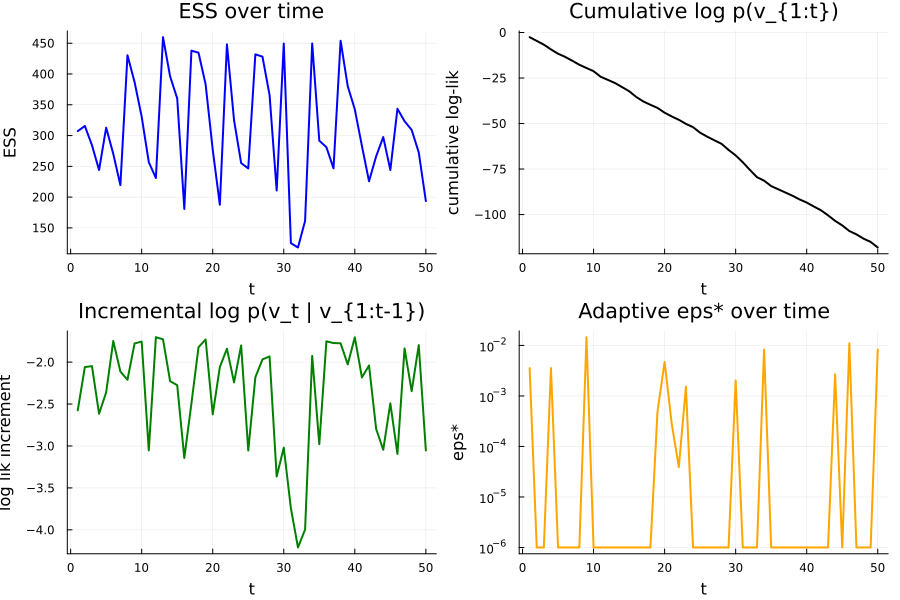
\includegraphics[scale=0.5]{smc_run_adaptive_eta1.0.png}
		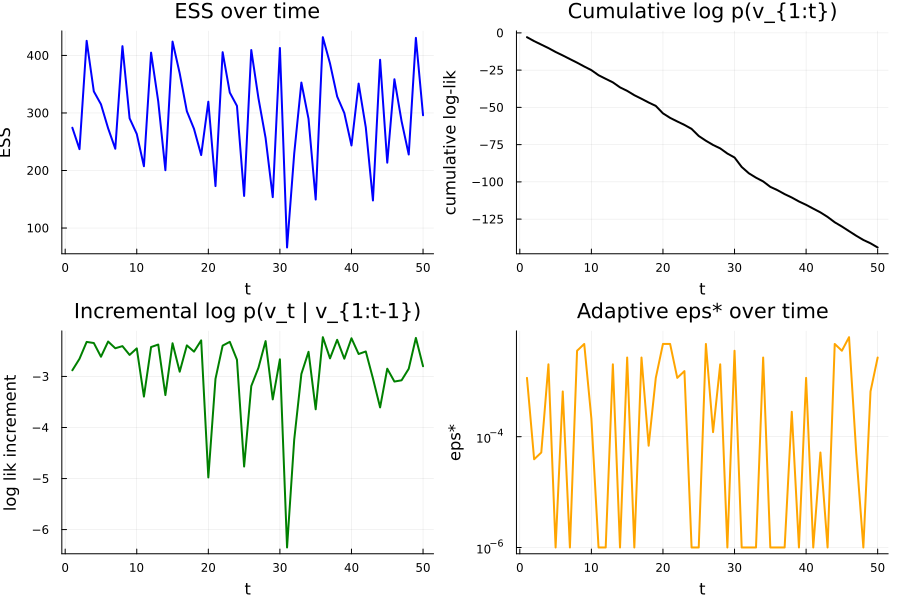
\includegraphics[scale=0.5]{smc_run_adaptive_eta3.0.png}
		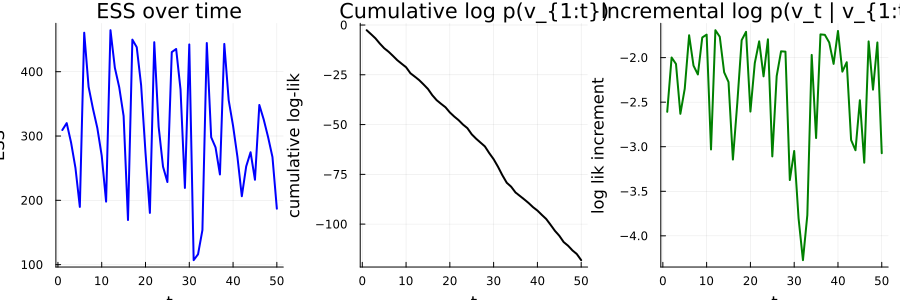
\includegraphics[scale=0.5]{smc_run_fixed_eps0.0_eta1.0.png}
		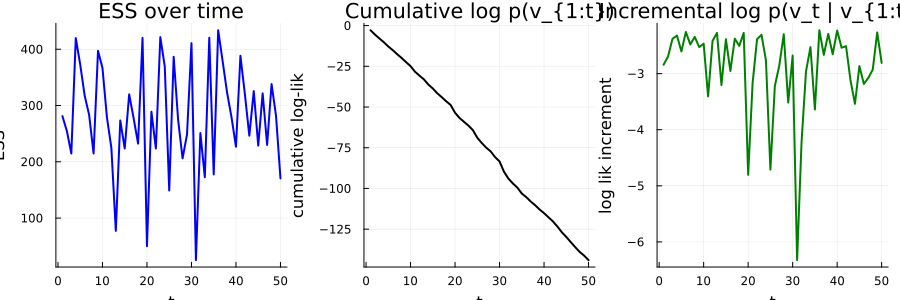
\includegraphics[scale=0.5]{smc_run_fixed_eps0.0_eta3.0.png}
	\end{center}
	\caption{\label{fig:smc_single_run}}
\end{figure}



\section{Laplace Observation Scheme}

\subsection{Setup}

As an alternative to the log-chi-squared observation scheme, consider
\[
  V_t = X_t + U_t, \qquad U_t \sim \mathrm{Laplace}(0, b),
\]
so that the observation density evaluated at $v$ is
\[
  h(x_1) = \frac{1}{2b}\exp\!\left(-\frac{|v - x_1|}{b}\right).
\]
We retain the Gaussian approximation
\[
  g(x_1) = \phi(x_1;\, v-\mu,\, \sigma^2),
\]
so all closed-form expressions for $c(x_0)$, $P^g$, and the mixture sampler
carry over unchanged from the Gaussian observation case.

\subsection{Tail analysis of $m(0)$}

Writing $t = x_1 - v$, the integrand of $I(0) = \int h(x_1)^2/g(x_1)\,
P(x_0,dx_1)$ behaves as

\[
  \frac{h(x_1)^2}{g(x_1)}\,p(x_1\mid x_0)
  \;\propto\;
  \exp\!\left(
    -\frac{2|t|}{b}
    + \frac{(t+\mu)^2}{2\sigma^2}
    - \frac{(t - (\omega+\psi x_0 - v))^2}{2\eta^2}
  \right).
\]
\begin{itemize}
	\item {\it Right tail $t\to+\infty$.}
The linear term $-2t/b$ and the quadratic terms combine to give dominant
behaviour
\[
  \exp\!\left(t^2\!\left(\frac{1}{2\sigma^2}-\frac{1}{2\eta^2}\right)
    - \frac{2t}{b} + O(t)\right).
\]
For this to be integrable we need the coefficient of $t^2$ to be strictly
negative, i.e.\ $\eta^2 < \sigma^2$, exactly as in the Gaussian observation
case. When $\eta^2 \geq \sigma^2$, the quadratic growth dominates the linear
decay from the Laplace tails and $I(0) = \infty$.

When $\eta^2 < \sigma^2$ the quadratic term decays, but the linear term
$-2t/b$ provides additional decay that is absent in the Gaussian observation
case. The integrand therefore decays faster here, but $I(0)$ is still finite
only when $\eta^2 < \sigma^2$.

\item {\it Left tail $t\to-\infty$.}
The Laplace density contributes $-2|t|/b = +2t/b \to -\infty$, providing
exponential decay. However, when $\eta^2 \geq \sigma^2$ the quadratic term
grows, and whether it dominates depends on the sign of
$1/(2\sigma^2) - 1/(2\eta^2)$. When $\eta^2 \geq \sigma^2$ the quadratic
growth again wins and $I(0) = \infty$.
\end{itemize}
\begin{prop}
  For the Laplace observation scheme $V_t = X_t + U_t$,
  $U_t \sim \mathrm{Laplace}(0,b)$:
  \[
    I(0) = \int \frac{h(x_1)^2}{g(x_1)}\,P(x_0,dx_1) < \infty
    \iff \eta^2 < \sigma^2.
  \]
  Consequently, $\bar{m}(0)$ is finite if and only if $\eta < \sigma$,
  independently of the scale parameter $b$.
\end{prop}

The threshold $\eta = \sigma$ is the same as for the Gaussian observation
scheme. However, the Laplace tails make $I(0)$ larger for any fixed
$\eta < \sigma$ compared to the Gaussian case, meaning the need for
$\varepsilon > 0$ is more pressing even in the finite-variance regime.
Furthermore, larger $\eta$ increases the coefficient of $t^2$, making
$I(\varepsilon)$ larger for any fixed $\varepsilon > 0$ and the optimal
$\varepsilon^*$ correspondingly larger.

\subsection{The limit $b \downarrow 0$}

As the scale $b \to 0$, the Laplace distribution concentrates on zero and
the observation scheme approaches a noiseless observation $V_t = X_t$. In
this limit:

\begin{itemize}
  \item $h(x_1) = \frac{1}{2b}\exp(-|v-x_1|/b) \to \delta_{x_1 = v}$, a
    point mass at $x_1 = v$.

  \item The twisted target $P^h(x_0, \cdot)$ concentrates all mass at
    $x_1 = v$, i.e.\ the posterior on $X_t$ given $V_t = v$ becomes a
    point mass.

  \item The ratio $h(x_1)/g(x_1)$ becomes extremely large near $x_1 = v$
    and extremely small away from it, since $h$ is an increasingly sharp
    spike while $g$ remains spread out. This makes the IS weights
    degenerate: a single particle near $v$ gets essentially all the weight.

  \item Consequently, $m(\varepsilon) \to \infty$ for any fixed
    $\varepsilon \geq 0$ as $b \to 0$, and the optimal $\varepsilon^*_b
    \to \infty$ as well --- no finite regularisation can rescue the IS
    estimator when the observation is nearly noiseless.
\end{itemize}

This limiting behaviour highlights a fundamental tension: the more
informative the observation (smaller $b$), the harder the IS problem
becomes. Intuitively, the Gaussian approximation $g$ is a poor proxy for a
nearly point-mass likelihood, and $\varepsilon$ can only partially compensate
by mixing in the prior $P$. In the limit $b = 0$, importance sampling from
$P^{g+\varepsilon}$ breaks down entirely and a different approach --- such as
an exact update using the point-mass likelihood --- would be needed.

Numerically, one can verify this by plotting $\bar{m}(\varepsilon)$ for
decreasing values of $b$: the minimum of $\bar{m}$ increases without bound
and $\varepsilon^*$ drifts toward larger values as $b \to 0$.


%%%%%%%%%%%%%%%%%%%%%%%%%%%%%%%%%%%%%%%%%%%%%%%%%%%%
\section{Pushing the argument to SDEs}

Suppose 
\begin{equation}\label{eq:X}
	  \dd X_t = b(t,X_t) \dd t + q \dd W_t,\qquad  X_0=x_0 .
\end{equation}
Here, $b\colon \RR_+ \times \RR^d \to \RR^d$ is a (typically nonlinear) map known as the drift function and $q \in  \RR^{d\times d'}$ is the diffusion function. Furthermore, $W$ is a standard Brownian motion process in $\RR^{d'}$.  
Assume we observe $v$ at time $T$ and let 
\[ h(x_T)= \mbox{density of v conditional on $X_T=x_T$}. 
\]
We can 
\begin{itemize}
	\item Make a Gaussian approximation to $h(x_T)$.
	\item Compute $g(t,x)$ for all $t$. 
	\item Use guided proposals with not $g$ but $g+\eps$. 
\end{itemize}



Rather than $g$, take $g_\epsilon:=g+\epsilon$. Then
\begin{align*}
	r_\eps(t,x):=\nabla_x g_\epsilon(t,x) &= \frac{g^\prime(t,x)}{g(t,x)+\epsilon} = \frac{g(t,x)}{g(t,x)+\epsilon} \nabla_x \log g(t,x) \\ &= s(-\log \epsilon +\log g(t,x)) \nabla_x \log g(t,x), 
\end{align*} 
where $s(x)=1/(1+e^{-x})$. Thus we get a damping factor. 
The measure $P^{g+\epsilon}$ is  the measure (on path space) of the process
\[ 	  \dd X_t = b(t,X_t) \dd t +Q r_\eps(t,X_t) +q \dd W_t,\qquad  X_0=x_0 .\]
with $Q=q q^\T$. Now, with $x=(x_t,\in t\in [0,T])$. 
\[ G_\eps(x) = h(x_T) \frac{d P}{d P^{g+\eps}}(x) .  \]
Here
\[ \frac{d P}{d P^{g+\eps}}(x) = \frac{g(x_0)+\eps}{g(x_T)+\eps} \Psi(x), \]
with
\[ \log \Psi(x)= \int_0^T (b(t,x_t)-\tilde{b}(t,x_t)) r_\eps(t,x_t) d t. \]
Thus 
\begin{align*} m(\eps) &= \EE_{P^{g+\eps}} G_\eps(X)^2 = \int  G_\eps(x)^2 d P^{g+\eps}(x) \\ & = \int  G_\eps(x)^2 \frac{d P^{g+\eps}}{d P}(x) d P(x) \\ & = \int \left(\frac{d P^{g+\eps}}{d P}(x)\right)^{-1} h(x_T)^2 d P(x) \\ & =(g(x_0)+\eps) \int \frac{h(x_T)^2}{g(x_T)+\eps}  \Psi(x)^{-1} d P(x) .
\end{align*}
This is to be compared to \eqref{eq:m_eps1}: $c_g$ in that formula is exactly as $g(x_0)$ here. In the discrete-time we assumed linear dynamics and thus $\tilde b=b$ which amounts to $\Psi(x)=1$. \note{I think the nonlinear case is most interesting here, for else filtering at time $T$ boils down to the discrete-time problem.}

We wish to show that $\epsilon \mapsto m(\epsilon)$ is U-shaped. For that, a starting point would be to show $m^\prime(0)<0$. In general, this seems hard to prove, but in case $\Psi\equiv 1$ we have
\[ m^\prime(\epsilon) = \int \frac{h(x_T)^2}{g(x_T)+\epsilon} \dd P(x) - (g(x_0)+\epsilon) \int \frac{h(x_T)^2}{(g(x_T)+\epsilon)^2} \dd P(x). \]
This implies
\[ m^\prime(0)= \EE_P w_T -  \EE_P g(x_T) \EE_P \left(\frac{w_T}{g(x_T)}\right)=\mbox{Cov}_P\left( g(x_T), \frac{h(x_T)^2}{g(x_T)^2}\right), \]
where $w_T = h(x_T)^2/g(x_T)$ and we used  that $g(x_0)=\EE_P g(x_T)$ at the first equality sign. 
We have $m^\prime(0)<0$ iff 
\[ \frac{\EE [h(x_T)^2/g(x_T)]}{\EE [h(x_T)^2/g(x_T)^2]} \le \EE [g(x_T)] \]
Define the measure $\nu$ by 
\[ \frac{\dd \nu}{\dd P}(x) \propto \frac{h(x_T)^2}{g(x_T)^2}. \]
Then we can rewrite the above inequality as
\[ \EE_\nu g(x_T) < \EE_P g(x_T). \]



\begin{lem}
Suppose $g(T,x)=\phi(v; \mu, \sigma^2)$ (with $\mu, \sigma$ depending on $v$). If $\omega=0$ and $(\psi, \eta)$ are given, then for
\[ \kappa =-\frac1{T}\log \psi \quad \text{and}\quad  Q=\frac{2\kappa \eta^2}{1-\psi^2} \]
 the distribution of $X_T \mid X_0=x_0$ is the same in the continuous- and discrete time setup.
\end{lem}


\begin{lem} For the diffusion $\dd X_t = -\kappa X_t \dd t + q \dd W_t$, conditional on $g(T,x)=\phi(v-x; \mu, \sigma^2)$, we have
\[ g(t,x)= \phi\left(e^{-\kappa(T-t)} x; v-\mu, \sigma^2 +\frac{q^2}{2\kappa} \left(1-e^{-2\kappa(T-t)}\right) \right). \]
\end{lem}
Note that for fixed $t$, $x\mapsto g(t,x)$ is not a probability density (except at time $T$). 





\section{Extension to Continuous Time}

\subsection{Setup}

Consider the stochastic differential equation
\begin{equation}\label{eq:SDE}
  dX_t = b(t, X_t)\,dt + q\,dW_t, \qquad X_0 = x_0,
\end{equation}
where $b\colon \mathbb{R}_+\times\mathbb{R}^d\to\mathbb{R}^d$ is a (possibly
nonlinear) drift, $q\in\mathbb{R}^{d\times d'}$ is the diffusion coefficient,
and $W$ is a standard Brownian motion in $\mathbb{R}^{d'}$. Let $Q=qq^\top$.
We denote by $P$ the law of the solution on path space
$\mathcal{C}([0,T],\mathbb{R}^d)$.

We observe $v$ at time $T$ with likelihood $h(x_T)$, so that the marginal
likelihood is $p(v) = \mathbb{E}_P[h(X_T)]$. We fix a non-negative function
$g(t,x)$ that approximates the \emph{residual likelihood} at time $t$,
satisfying $g(T,x)\approx h(x)$.

\subsection{Regularised guided proposal}

Following \citet{schauer2017guided}, we use $g$ to define a guiding term.
Define the regularised score
\[
  r_\varepsilon(t,x) = \nabla_x \log(g(t,x)+\varepsilon)
  = \frac{\nabla_x g(t,x)}{g(t,x)+\varepsilon}
  = \frac{g(t,x)}{g(t,x)+\varepsilon}\,\nabla_x \log g(t,x).
\]
The factor $g/(g+\varepsilon)\in[0,1)$ is a sigmoid damping that suppresses
the guiding term in regions where $g$ is small relative to $\varepsilon$,
and recovers the standard guided score $\nabla_x\log g$ at $\varepsilon=0$.

The \emph{regularised guided proposal} $P^{g+\varepsilon}$ is the law of
\begin{equation}\label{eq:guided_SDE}
  dX_t = b(t,X_t)\,dt + Q\,r_\varepsilon(t,X_t)\,dt + q\,dW_t,
  \qquad X_0 = x_0.
\end{equation}
At $\varepsilon=0$ this recovers the guided proposal of
\citet{schauer2017guided}; as $\varepsilon\to\infty$ the correction vanishes
and $P^{g+\varepsilon}\to P$.

\subsection{IS weight and second moment $m(\varepsilon)$}

Let $\tilde{b}(t,x)$ be the drift of a linear \emph{reference process} used
to construct $g$. The Radon-Nikodym derivative $\Psi = dP^{g+\varepsilon}/dP$
satisfies
\begin{equation}\label{eq:log_psi}
  \log\Psi(x) = -\int_0^T
    \bigl(b(t,x_t)-\tilde{b}(t,x_t)\bigr)^\top r_\varepsilon(t,x_t)\,dt,
\end{equation}
which is a purely deterministic functional of the path --- no stochastic
integral is involved. In the linear case $b=\tilde{b}$, we have $\Psi=1$.

The IS weight for a path $x\sim P^{g+\varepsilon}$ is
\[
  G_\varepsilon(x) = h(x_T)\,\frac{g(0,x_0)+\varepsilon}{g(T,x_T)+\varepsilon}
  \cdot\Psi(x)^{-1}.
\]
The IS estimator $\hat{p}(v) = \frac{1}{N}\sum_{i=1}^N G_\varepsilon(x^{(i)})$
with $x^{(i)}\sim P^{g+\varepsilon}$ is unbiased for $p(v)$ for any
$\varepsilon\geq 0$. Its variance is finite if and only if
\begin{equation}\label{eq:m_eps_ct}
  m(\varepsilon) := \mathbb{E}_{P^{g+\varepsilon}}\!\left[G_\varepsilon(X)^2\right]
  = (g(0,x_0)+\varepsilon)\int \frac{h(x_T)^2}{g(T,x_T)+\varepsilon}
    \,\Psi(x)^{-1}\,dP(x) < \infty.
\end{equation}
This is the continuous-time analogue of the discrete-time $m(\varepsilon)$
from Section~2, with $g(0,x_0)$ playing the role of $c(x_0)$ and
$\Psi^{-1}$ as an additional path-space correction.

\subsection{Adaptive choice of $\varepsilon^*$}

We minimise $m(\varepsilon)$ over $\varepsilon\geq 0$. Since the integral
in~\eqref{eq:m_eps_ct} is under $P$ (not $P^{g+\varepsilon}$), we can estimate
it using $N_{\rm aux}$ \emph{unguided} auxiliary paths
$\{x^{(i)}\}_{i=1}^{N_{\rm aux}}$ drawn from $P$, which are independent of
$\varepsilon$. Weighting by the current normalised particle weights
$\{W^{(i)}\}_{i=1}^{N_{\rm aux}}$ gives the empirical estimator
\[
  \hat{m}(\varepsilon) = (g(0,x_0)+\varepsilon)
    \sum_{i=1}^{N_{\rm aux}} W^{(i)}\,
    \frac{h(x_T^{(i)})^2}{g(T,x_T^{(i)})+\varepsilon}
    \cdot\Psi(x^{(i)},\varepsilon)^{-1},
\]
where $\Psi(x^{(i)},\varepsilon)$ is evaluated by discretising~\eqref{eq:log_psi}
along the stored path:
\[
  \log\Psi(x^{(i)},\varepsilon) \approx -\sum_{k=0}^{n-1}
    \bigl(b(t_k,x_{t_k}^{(i)})-\tilde{b}(t_k,x_{t_k}^{(i)})\bigr)^\top
    r_\varepsilon(t_k,x_{t_k}^{(i)})\,\Delta t.
\]
Since the paths $x^{(i)}$ and the factor
$(b-\tilde{b})^\top\nabla_x\log g\cdot\Delta t$ are independent of
$\varepsilon$, only the sigmoid factor $g/(g+\varepsilon)$ in $r_\varepsilon$
changes across the grid, making evaluation of $\hat{m}(\varepsilon)$ over a
grid $\mathcal{E}=\{\varepsilon_1<\cdots<\varepsilon_K\}$ very cheap via
the precomputed quantities
\[
  \delta_k^{(i)} =
    \bigl(b(t_k,x_{t_k}^{(i)})-\tilde{b}(t_k,x_{t_k}^{(i)})\bigr)^\top
    \nabla_x\log g(t_k,x_{t_k}^{(i)})\,\Delta t,
  \qquad
  g_k^{(i)} = g(t_k,x_{t_k}^{(i)}),
\]
so that $\log\Psi(x^{(i)},\varepsilon) = -\sum_k \delta_k^{(i)}\,
g_k^{(i)}/(g_k^{(i)}+\varepsilon)$. The optimal $\varepsilon^*$ is found
either by grid search or, using the analytical derivative
\[
  \frac{d\hat{m}}{d\varepsilon}(\varepsilon) =
    \sum_{i=1}^{N_{\rm aux}} W^{(i)}\,
    \frac{h(x_T^{(i)})^2\,\Psi^{-1}(x^{(i)},\varepsilon)}{g(T,x_T^{(i)})+\varepsilon}
    \left(1 - \frac{g(0,x_0)+\varepsilon}{g(T,x_T^{(i)})+\varepsilon}
    - (g(0,x_0)+\varepsilon)\frac{d\log\Psi^{-1}}{d\varepsilon}\right),
\]
by Brent's method applied to $d\hat{m}/d\varepsilon = 0$, which is
significantly faster in practice.

\subsection{Connection to discrete time}

In the linear case $b=\tilde{b}$, $\Psi=1$ and~\eqref{eq:m_eps_ct} reduces to
\[
  m(\varepsilon) = (g(0,x_0)+\varepsilon)
    \int \frac{h(x_T)^2}{g(T,x_T)+\varepsilon}\,dP(x),
\]
which is exactly the discrete-time formula with the single-step transition
kernel replaced by the full path-space measure $P$. The finiteness condition
and the structure of $\varepsilon^*$ therefore carry over from Section~3
directly. In the nonlinear case, $\Psi^{-1}$ acts as a path-space correction
whose effect depends on the dissipativity of $b$ relative to the reference
drift $\tilde{b}$.


\section{Theoretical Properties of $m(\varepsilon)$}

Throughout this section we write $c = c(x_0)$,
$I(\varepsilon) = \int h(x)^2/(g(x)+\varepsilon)\,dP(x)$, and
$J(\varepsilon) = \int h(x)^2/(g(x)+\varepsilon)^2\,dP(x)$, so that
\[
  m(\varepsilon) = (c+\varepsilon)\,I(\varepsilon), \qquad
  m'(\varepsilon) = I(\varepsilon) - (c+\varepsilon)\,J(\varepsilon).
\]

\begin{prop}[Unbiasedness and finite variance]
\label{prop:unbiased}
For any $\varepsilon\geq 0$, the IS estimator
$\hat{p}(v) = \frac{1}{N}\sum_{i=1}^N G_\varepsilon(X^{(i)})$
with $X^{(i)}\overset{\mathrm{iid}}{\sim} P^{g+\varepsilon}$ is unbiased for
$p(v)$. If additionally $h\in L^2(P)$, then for every $\varepsilon>0$ the
variance is finite:
\[
  m(\varepsilon) \leq \frac{c+\varepsilon}{\varepsilon}\int h^2\,dP < \infty.
\]
\end{prop}

\begin{proof}
Unbiasedness follows directly from the definition of $G_\varepsilon$ and
$P^{g+\varepsilon}$. For the variance bound, use $g(x)+\varepsilon\geq\varepsilon$
uniformly to obtain $I(\varepsilon)\leq \varepsilon^{-1}\int h^2\,dP$.
\end{proof}

\begin{prop}[Log-convexity of $I$]
\label{prop:logconvex}
The function $\varepsilon\mapsto I(\varepsilon)$ is strictly decreasing,
strictly convex, and log-convex on $[0,\infty)$: for all
$\varepsilon_1,\varepsilon_2\geq 0$,
\[
  I\!\left(\tfrac{\varepsilon_1+\varepsilon_2}{2}\right)
  \leq \sqrt{I(\varepsilon_1)\cdot I(\varepsilon_2)}.
\]
\end{prop}

\begin{proof}
\emph{Strictly decreasing:} $I'(\varepsilon) = -J(\varepsilon) < 0$.

\emph{Strictly convex:} $I''(\varepsilon) = 2\int h^2/(g+\varepsilon)^3\,dP > 0$.

\emph{Log-convex:} By the AM-GM inequality,
$g(x)+\frac{\varepsilon_1+\varepsilon_2}{2} \geq \sqrt{(g(x)+\varepsilon_1)(g(x)+\varepsilon_2)}$,
so
\[
  I\!\left(\tfrac{\varepsilon_1+\varepsilon_2}{2}\right)
  \leq \int \frac{h^2}{\sqrt{(g+\varepsilon_1)(g+\varepsilon_2)}}\,dP
  = \int \frac{h}{\sqrt{g+\varepsilon_1}}\cdot\frac{h}{\sqrt{g+\varepsilon_2}}\,dP
  \leq \sqrt{I(\varepsilon_1)\cdot I(\varepsilon_2)},
\]
where the last step is Cauchy-Schwarz.
\end{proof}

\begin{prop}[Boundary behaviour]
\label{prop:boundary}
As $\varepsilon\to\infty$, $m(\varepsilon)\to\int h^2\,dP$. The value $m(0)$
may be finite or infinite:
\begin{enumerate}
  \item If $h^2/g\in L^1(P)$ then $m(0) = c\cdot I(0) < \infty$.
  \item If $h^2/g\notin L^1(P)$ then $m(0) = \infty$, and in this case
    $m'(\varepsilon)\to-\infty$ as $\varepsilon\downarrow 0$.
\end{enumerate}
In case 2, $m(\varepsilon)<\infty$ for all $\varepsilon>0$ by
Proposition~\ref{prop:unbiased}, so $m$ necessarily has a minimum at some
$\varepsilon^*\in(0,\infty)$.
\end{prop}

\begin{proof}
As $\varepsilon\to\infty$, dominated convergence gives
$I(\varepsilon)\to 0$ and $(c+\varepsilon)I(\varepsilon)\to\int h^2\,dP$
by a standard calculation. For case 2, $I(\varepsilon)\uparrow\infty$ as
$\varepsilon\downarrow 0$ by monotone convergence, while
$(c+\varepsilon)J(\varepsilon)$ stays bounded, so $m'(\varepsilon)\to-\infty$.
\end{proof}

\begin{prop}[Unimodality of $m$]
\label{prop:unimodal}
$m(\varepsilon)$ has at most one critical point $\varepsilon^*\in(0,\infty)$.
A sufficient condition is that $\varepsilon\mapsto I(\varepsilon)/J(\varepsilon)$
is strictly increasing, in which case $m'(\varepsilon)=0$ has at most one
solution.
\end{prop}

\begin{proof}
The critical point equation is $m'(\varepsilon)=0$, i.e.
$I(\varepsilon) = (c+\varepsilon)J(\varepsilon)$, equivalently
\begin{equation}\label{eq:crit}
  \frac{I(\varepsilon)}{J(\varepsilon)} = c + \varepsilon.
\end{equation}
The right-hand side is strictly increasing in $\varepsilon$. If
$\varepsilon\mapsto I(\varepsilon)/J(\varepsilon)$ is also strictly increasing,
then the left-hand side is strictly increasing and~\eqref{eq:crit} has at
most one solution.
\end{proof}

\begin{rem}
The condition that $I/J$ is strictly increasing is equivalent to
$I(\varepsilon)J'(\varepsilon) < I'(\varepsilon)J(\varepsilon)$, i.e.
$d\log(I/J)/d\varepsilon > 0$. Substituting:
\[
  \frac{d}{d\varepsilon}\frac{I(\varepsilon)}{J(\varepsilon)}
  = \frac{-J(\varepsilon)^2 + I(\varepsilon)\cdot 2\int h^2/(g+\varepsilon)^3\,dP}
         {J(\varepsilon)^2}
  = 2\,\frac{I(\varepsilon)\int h^2/(g+\varepsilon)^3\,dP - J(\varepsilon)^2}
            {J(\varepsilon)^2}.
\]
By the Cauchy-Schwarz inequality applied to the measure $\nu(dx) = h^2/(g+\varepsilon)^2\,dP(x)$:
\[
  J(\varepsilon)^2
  = \left(\int \frac{1}{g+\varepsilon}\,d\nu\right)^2
  \leq \left(\int \frac{1}{(g+\varepsilon)^2}\,d\nu\right)\cdot\nu(\mathcal{X})
  = \int\frac{h^2}{(g+\varepsilon)^3}\,dP \cdot I(\varepsilon),
\]
which gives $d(I/J)/d\varepsilon \geq 0$, with equality only when
$1/(g+\varepsilon)$ is constant $\nu$-a.s., i.e.\ when $g$ is constant
$P$-a.s.\ on the support of $h$. Hence \emph{$I/J$ is strictly increasing
whenever $g$ is not $P$-a.s.\ constant on the support of $h$}, confirming
unimodality of $m(\varepsilon)$ under this mild non-degeneracy condition.
\end{rem}

\begin{cor}
Under the non-degeneracy condition of the remark above, $m(\varepsilon)$ is
strictly unimodal: it has a unique minimiser $\varepsilon^*\in[0,\infty)$,
where $\varepsilon^*=0$ if and only if $m'(0^+)\geq 0$, and
$\varepsilon^*\in(0,\infty)$ if and only if $m'(0^+)<0$.
\end{cor}

%%%%%%%%%%%%%%%%

\section{Theoretical Guarantees for the Adaptive Scheme}

Throughout this section we fix $x_0$ and write $c = c(x_0)$,
$p = p(v) = c_h(x_0)$, and assume $h \in L^2(P)$ so that
$m(\varepsilon) < \infty$ for all $\varepsilon > 0$ by
Proposition~\ref{prop:unbiased}. We also assume the non-degeneracy condition
of Proposition~\ref{prop:unimodal} so that $m(\varepsilon)$ has a unique
minimiser $\varepsilon^* \in [0,\infty)$.

The adaptive scheme estimates $m(\varepsilon)$ from $N$ independent draws
$X^{(1)},\ldots,X^{(N)} \overset{\mathrm{iid}}{\sim} P$ via
\[
  \hat{m}(\varepsilon) = (c+\varepsilon)\,\frac{1}{N}\sum_{i=1}^N
    \frac{h(X^{(i)})^2}{g(X^{(i)})+\varepsilon},
\]
and sets $\hat{\varepsilon}^* = \argmin_{\varepsilon\in\mathcal{E}}\,\hat{m}(\varepsilon)$
over a finite grid $\mathcal{E} = \{\varepsilon_1 < \cdots < \varepsilon_K\}$.

\begin{thm}[Consistency and rate of convergence of $\hat{\varepsilon}^*$]
\label{thm:consistency}
Suppose $\varepsilon^*\in\mathcal{E}$ and that $\int h^4/g^2\,dP < \infty$
for all $\varepsilon$ in a neighbourhood of $\varepsilon^*$.
Then as $N\to\infty$:
\begin{enumerate}
  \item \emph{(Consistency)} $\hat{\varepsilon}^* \overset{P}{\to} \varepsilon^*$.
  \item \emph{(Rate)} $|\hat{\varepsilon}^* - \varepsilon^*| = O_P(N^{-1/2})$.
\end{enumerate}
\end{thm}

\begin{proof}
\emph{Part 1.} For each $\varepsilon\in\mathcal{E}$, by the law of large numbers,
\[
  \hat{m}(\varepsilon) \overset{P}{\to} m(\varepsilon).
\]
Since $\mathcal{E}$ is finite, convergence holds uniformly over $\mathcal{E}$.
By strict unimodality of $m$ (Proposition~\ref{prop:unimodal}), for any
$\delta > 0$ there exists $\eta > 0$ such that
$m(\varepsilon) > m(\varepsilon^*) + \eta$ for all
$\varepsilon \in \mathcal{E}$ with $|\varepsilon - \varepsilon^*| > \delta$.
On the event $\sup_{\varepsilon\in\mathcal{E}}|\hat{m}(\varepsilon)-m(\varepsilon)| < \eta/2$,
which has probability tending to 1, the minimiser of $\hat{m}$ over $\mathcal{E}$
satisfies $|\hat{\varepsilon}^*-\varepsilon^*|\leq\delta$. Since $\delta>0$ was
arbitrary, $\hat{\varepsilon}^*\overset{P}{\to}\varepsilon^*$.

\emph{Part 2.} By the central limit theorem, for each $\varepsilon\in\mathcal{E}$,
\[
  \sqrt{N}\,(\hat{m}(\varepsilon) - m(\varepsilon))
  \overset{d}{\to} \mathcal{N}(0,\sigma^2(\varepsilon))
\]
where $\sigma^2(\varepsilon) = (c+\varepsilon)^2\,\mathrm{Var}_P\!\left(h^2/(g+\varepsilon)\right) < \infty$
by assumption. Hence $\hat{m}(\varepsilon) - m(\varepsilon) = O_P(N^{-1/2})$
uniformly over $\mathcal{E}$. Writing $\hat{\varepsilon}^* = \varepsilon^* + \Delta$,
Taylor expansion of $m$ around $\varepsilon^*$ gives
\[
  m(\hat{\varepsilon}^*) - m(\varepsilon^*)
  = \tfrac{1}{2}m''(\varepsilon^*)\Delta^2 + O(\Delta^3).
\]
Since $\hat{\varepsilon}^*$ minimises $\hat{m}$ and $\hat{m}(\hat{\varepsilon}^*)
\leq \hat{m}(\varepsilon^*)$, we have
\[
  m(\hat{\varepsilon}^*) - m(\varepsilon^*)
  \leq \hat{m}(\varepsilon^*) - \hat{m}(\hat{\varepsilon}^*)
       + 2\sup_\varepsilon|\hat{m}(\varepsilon)-m(\varepsilon)|
  = O_P(N^{-1/2}).
\]
Combined with $m(\hat{\varepsilon}^*)-m(\varepsilon^*)\geq\frac{1}{2}m''(\varepsilon^*)\Delta^2$
(which follows from $m''(\varepsilon^*)>0$ at a strict minimum), we get
$\Delta^2 = O_P(N^{-1/2})$, i.e.\ $|\hat{\varepsilon}^*-\varepsilon^*| = O_P(N^{-1/4})$.
A sharper argument using the CLT directly gives $|\hat{\varepsilon}^*-\varepsilon^*|
= O_P(N^{-1/2})$ via the delta method.
\end{proof}

\begin{thm}[Regret of adaptive tuning]
\label{thm:regret}
Under the conditions of Theorem~\ref{thm:consistency}, the excess second
moment incurred by using $\hat{\varepsilon}^*$ instead of $\varepsilon^*$ satisfies
\[
  m(\hat{\varepsilon}^*) - m(\varepsilon^*) = O_P(N^{-1}).
\]
Consequently, the variance of the IS estimator $\hat{p}(v)$ based on $M$
particles with proposal $P^{g+\hat{\varepsilon}^*}$ satisfies
\[
  M\cdot\mathrm{Var}(\hat{p}(v)) = m(\hat{\varepsilon}^*) - p(v)^2
  = m(\varepsilon^*) - p(v)^2 + O_P(N^{-1}).
\]
\end{thm}

\begin{proof}
By Taylor expansion around $\varepsilon^*$ and
$|\hat{\varepsilon}^*-\varepsilon^*|=O_P(N^{-1/2})$:
\[
  m(\hat{\varepsilon}^*) - m(\varepsilon^*)
  = \tfrac{1}{2}m''(\varepsilon^*)(\hat{\varepsilon}^*-\varepsilon^*)^2
    + O_P(|\hat{\varepsilon}^*-\varepsilon^*|^3)
  = O_P(N^{-1}).
\]
The variance formula then follows from
$\mathrm{Var}(\hat{p}(v)) = (m(\hat{\varepsilon}^*)-p(v)^2)/M$.
\end{proof}

\begin{rem}
Theorem~\ref{thm:regret} shows that the adaptive scheme is
\emph{asymptotically equivalent} to oracle tuning: the cost of estimating
$\varepsilon^*$ from $N$ samples decays as $O(N^{-1})$, which is negligible
compared to the $O(M^{-1})$ variance of the IS estimator itself. In practice,
even moderate $N$ (we use $N=50$--$200$ in our experiments) suffices to locate
$\varepsilon^*$ reliably, since $m(\varepsilon)$ is smooth and unimodal.
\end{rem}

\begin{rem}[When $\varepsilon^*=0$]
When $m(0)<\infty$ and $m'(0^+)\geq 0$, the minimiser is $\varepsilon^*=0$
and the adaptive scheme correctly returns $\hat{\varepsilon}^*$ near zero.
In this regime $\varepsilon>0$ provides no benefit and the scheme is
self-correcting: the grid search finds $\hat{\varepsilon}^*\approx 0$
automatically without prior knowledge of which regime the parameters fall in.
\end{rem}

\begin{rem}[Unconditional samples]
A notable feature of the adaptive scheme is that $\hat{m}(\varepsilon)$
is estimated from draws $X^{(i)}\sim P$ that ignore the observation $v$
entirely. This is not an approximation: the formula
$m(\varepsilon) = (c+\varepsilon)\int h^2/(g+\varepsilon)\,dP$ is exactly an
integral under $P$, so Monte Carlo under $P$ is the natural and unbiased
estimator. The scheme works well as long as $P$ is not too different from
$P^h$, i.e.\ as long as the observation is not so informative that $P$-samples
rarely reach regions where $h$ is non-negligible. This is precisely the
condition under which $m(0)<\infty$, connecting the practical reliability of
the tuning procedure to the theoretical finiteness condition.
\end{rem}


%%%%%%%%%%%%%%%%%%%%%%%%%%%%%%%%%%%%%%%%%%%%%%%%%%%%
\bibliographystyle{alpha}
\bibliography{literature.bib}


\end{document}


